%%%%%%%%%%%%%%%%%%%%%%%%%%%%%%%%%%%%%%%%%%%%%%%%%%%%%%%%%%%%%%%%%%%%
%% I, the copyright holder of this work, release this work into the
%% public domain. This applies worldwide. In some countries this may
%% not be legally possible; if so: I grant anyone the right to use
%% this work for any purpose, without any conditions, unless such
%% conditions are required by law.
%%%%%%%%%%%%%%%%%%%%%%%%%%%%%%%%%%%%%%%%%%%%%%%%%%%%%%%%%%%%%%%%%%%%

\documentclass{beamer}
\usetheme[faculty=fi, locale=czech]{fibeamer}
\usepackage[utf8]{inputenc}
\usepackage[czech]{babel}
\usepackage{tabularx, booktabs}

\input{resources/header.tex}


%% These macros specify information about the presentation
\title{Verifikace binarizovaných neuronových sítí pomocí ASP} %% that will be typeset on the
\subtitle{Obhajoba bakalářské práce} %% title page.
\author{Jindřich Matuška}

%% These additional packages are used within the document:
%\usepackage{ragged2e}    % `\justifying` text
%\usepackage{booktabs}    % Tables
%\usepackage{tabularx}
%\usepackage{tikz}        % Diagrams
%\usetikzlibrary{calc,positioning}
%\usepackage{svg}
%\usetikzlibrary{calc, shapes, backgrounds}
%\usepackage{amsmath, amssymb}
%\usepackage{url}         % `\url`s
%\usepackage{listings}    % Code listings
%\frenchspacing

%\usepackage{pgfplots}
%\usetikzlibrary{plotmarks}


\newcommand{\style}{}

% bachelor thesis stylesheet
\newcommand{\itonly}[2]{%
    \only<#1>{%
        \begin{itemize}%
            \item #2%
        \end{itemize}%
    }%
}

\newcommand{\sign}{\text{sign}}

\newcommand{\icon}[1]{
    \begin{tikzpicture}[overlay,remember picture]%
        \node[anchor=north east,xshift=-30pt, yshift=-24pt]%
            at (current page.north east) {%
                \includegraphics[height=20mm]{resources/#1\style}%
            };%
    \end{tikzpicture}%
}

% chktex-file 1

\begin{document}
    \shorthandoff{-}
    \frame[c]{\maketitle}

    \AtBeginSection[]{% Print an outline at the beginning of sections
        \begin{frame}<beamer>
            \frametitle{Obsah}
            \tableofcontents[currentsection]
        \end{frame}}

    \begin{frame}<beamer>
        \frametitle{Obsah}
        \tableofcontents
    \end{frame}
    
    \section{Binarizovaná neuronová síť}
    % \subsection{Binarizovaná neuronová síť}
    \begin{frame}{Binarizovaná neuronová síť}
        \begin{itemize}
            \item Hluboká neuronová síť

\vspace{1em}
                \only<1>{
\begin{figure}[h]
    \begin{center}
        \scalebox{0.5}{
    \begin{tikzpicture}
        \setupnodes{(0,0)}
        \valuenode{1}
        \valuenode{x_1}
        \valuenode{x_2}
        \node (lastNode) at ($(lastNode.south) + (0,-1)$) {};
        \valuenode{x_{n_0}}
        \draw[thick,dotted,shorten <= 1em,shorten >= 1em] (x_2) -- (x_{n_0});
        
        \setupnodes{($(1.east) + (3,0)$)}
        \valuenode{1{}}
        \percnode{1/1}{1/,x_1/,x_2/,x_{n_0}/}
        \percnode{1/2}{1/,x_1/,x_2/,x_{n_0}/}
        \node (lastNode) at ($(lastNode.south) + (0,-1)$) {};
        \percnode{1/n_1}{1/,x_1/,x_2/,x_{n_0}/}
        \draw[thick,dotted,shorten <= 1em,shorten >= 1em] (p{1/2}) -- (p{1/n_1});
        \setupnodes{(1{}.east)}
        \valuenode{1}

        \setupnodes{($(1.east) + (3,0)$)}
        \valuenode{1{}}
        \percnode{2/1}{1/,p{1/1}/,p{1/2}/,p{1/n_1}/}
        \percnode{2/2}{1/,p{1/1}/,p{1/2}/,p{1/n_1}/}
        \node (lastNode) at ($(lastNode.south) + (0,-1)$) {};
        \percnode{2/n_2}{1/,p{1/1}/,p{1/2}/,p{1/n_1}/}
        \draw[thick,dotted,shorten <= 1em,shorten >= 1em] (p{2/2}) -- (p{2/n_2});
        \setupnodes{(1{}.east)}
        \valuenode{1}

        \setupnodes{($(p{2/1}.east) + (3.5,0)$)}
        \amnode[dotted]{d+1/1}{1/,p{2/1}/,p{2/2}/,p{2/n_2}/}
        \amnode[dotted]{d+1/2}{1/,p{2/1}/,p{2/2}/,p{2/n_2}/}
        \node (lastNode) at ($(lastNode.south) + (0,-1)$) {};
        \amnode[dotted]{d+1/n_{d+1}}{1/,p{2/1}/,p{2/2}/,p{2/n_2}/}
        \draw[thick,dotted,shorten <= 1em,shorten >= 1em] (p{d+1/2}) -- (p{d+1/n_{d+1}});

        \setupnodes{($(p{d+1/1}.east) + (2,0)$)}
        \valuenode{y_1}
        \setupnodes{($(p{d+1/2}.east) + (2,0)$)}
        \valuenode{y_2}
        \setupnodes{($(p{d+1/n_{d+1}}.east) + (2,0)$)}
        \valuenode{y_{n_{d+1}}}
        \draw[thick,dotted,shorten <= 1em,shorten >= 1em] (y_2) -- (y_{n_{d+1}});

        \draw (p{d+1/1}.east) -- (y_1.west);
        \draw (p{d+1/2}.east) -- (y_2.west);
        \draw (p{d+1/n_{d+1}}.east) -- (y_{n_{d+1}}.west);
    \end{tikzpicture}
        }
    \end{center}
\end{figure}
\vspace{-2em}
                }

            \item Perceptron
                \only<2>{
                \[p = H\circ \xi,\, \hat p = H\circ \rho\circ \xi\]
                \[\xi (\vec x) = b + \sum_i w_i\cdot x_i,\, b\in \RR,\, w_i\in\BB\]
                \vspace{-1em}
                \[\rho(x) = \alpha\cdot \left({x-\mu \over \sigma}\right),\hspace{1em} H(x) = \begin{cases}1 & x \geq 0\\ -1 & \text{jinak}\end{cases}\]
            }
            \item Argmax vrstva
        \end{itemize}
    \end{frame}

    \subsection{Robustnost binarizované neuronové sítě}
    \begin{frame}{Robustnost funkce}

        \begin{itemize}
            \item Kvantitativní definice robustnosti
                \itonly{1-}{Hodnocená funkce $F: P\to Q$}
                \itonly{1-}{Oblast vstupů $I \subseteq P$}
                \itonly{1-}{Funkce vah vstupů $w: P\to \RR,\, \forall x\in I: w(x) > 0$}
                \itonly{1-}{Hodnotící funkce $h_p: Q \to [0, 1],\, h_p(F(p)) = 0$}

    \begin{equation*}
        Q_{w, h_p}(I) = \frac{\sum_{i\in I} w(i)\cdot h_p(F(i))}{\sum_{i\in I} w(i)}
    \end{equation*}
            \item Kvalitativní definice robustnosti
                \[Q_{w, h_p}(I) = 0 \iff \forall i\in I.\, h_p(F(i)) = 0\]
        \end{itemize}
    \end{frame}

    \begin{frame}{Oblasti vstupů}
        \begin{itemize}
            \item Oblast vstupů
                \itonly{1-}{podle Hammingovy vzdálenosti $r$}
                \[R(\vec x, r) = \{\vec u \mid HD(\vec x, \vec u) \leq r\}\]
                \[\|R(\vec x, r)\| = \sum_{i=0}^{r} {n_0\choose i}\]
                \itonly{1-}{podle pevně zvolených pozic $F \subseteq \{1, \ldots, n_0\}$}
                \[R(\vec x, F) = \{\vec u \mid \forall i\in F.\, x_i = u_i\}\]
                \[\|R(\vec x, F)\| = 2^{n_0-\|F\|}\]
        \end{itemize}
    \end{frame}

    \section{Answer set programming}
    \begin{frame}{Answer set programming}
        \begin{itemize}
            \item Deklarativní programovací paradigma
            \item Vhodné pro prohledávací problémy
            \item Pravidla ve formě
                \itonly{1-}{\asprule{l_0\, or\, \ldots\, or\, l_k}{l_{k+1}, \ldots, l_{m}, \aspnot l_{m+1}, \ldots, \aspnot l_{n}}}
                % Odstranit / posunout do diskuze?
            \item Klasická negace (součást literálu) $\neg$ vs.\ negace jako selhání $\aspnot$
            \item Konzistence parciální interpretace s pravidlem
        \end{itemize}
    \end{frame}

    \subsection{Clingo framework}
    \begin{frame}{Clingo framework}
        \begin{itemize}
            \item Gringo, Clasp
            \item Rozšíření ASP
                \itonly{1-}{Parametrizované atomy a pravidla (pouze celočíselné parametry)}
                \itonly{1-}{Agregátní funkce nad množinami (součet, počet, maximum, \ldots)}
            % Odstranit?
            \item Grounding --- převod do mezijazyka aspif
                \itonly{1-}{Jazyk bez parametrů}
                \itonly{1-}{Každý \textbf{možný} literál reprezentuje unikátní přirozené číslo}
            \item Solving --- hledání řešení
                \itonly{1-}{Zařezávání větví}
                \itonly{1-}{Nutnost projít všechna řešení (enumerace modelů)}
        \end{itemize}
    \end{frame}

    \section{Přepis BNN do jazyka Clingo}
    % TODO Here

    \subsection{Transformace binarizované neuronové sítě pro Clingo}
    \begin{frame}{Transformace neuronové sítě}
        \begin{itemize}
            \item Kódování BNN pomocí celých čísel
                \only<1>{
                    \[
	(H \circ \rho \circ \xi)(\vec x) \equiv \alpha\cdot \left(\frac{
		b + \sum_{i=1}^k w_i\cdot x_i
	-\mu}{\sigma}\right) + \gamma \geq 0
                    \]
                    \[
    b' = \pm\left(-b +\mu - \frac{\sigma\cdot \gamma}{\alpha}\right), \vec w' = \pm\vec w
                    \]
                    \[
                        (H \circ \rho \circ \xi)(\vec x) \equiv \sum_{i=1}^k w_i'\cdot x_i \geq \floor{b'}
                    \]
                }
            \item Výstupní blok
            \item Transformace pomocí jazyka Python
        \end{itemize}
    \end{frame}

    \subsection{Kódování v jazyce Clingo}
    \begin{frame}{Kódování problému}
        \begin{itemize}
            \item Oblast vstupů
                \itonly{1}{Hamingova vzdálenost

                \texttt{%
                    \{on(0, 1..N)\} :- layer(0, N).\\
                    :- \#count \{ N : not input(N), on(0, N);\\
           \phantom{aaaaaaaaaaaa}N : input(N), not on(0, N) \} > H,\\
           \phantom{aaaa}hamdist(H).
                }}
                \itonly{1}{Fixní hodnoty pozic

                \texttt{%
                    on(0, N) :- input(N), inpfix(N).\\
                    \{on(0, K)\} :- not inpfix(K), layer(0, N), K=1..N.
                }}
            \item Vnitřní vrstvy
                \itonly{2}{Bez ukládání mezivýsledků $\xi(\vec x)$}

                \only<2>{
                    \texttt{on(L, N) :-\\
                        \#sum\{W,I: on(L-1, I), weight(L, I, N, W)\} >= B,\\
                        bias(L, N, B), not output\_layer(L).}
                    }
            \item Výstupní vrstva
                \itonly{3}{Zneplatnění modelů s očekávaným výstupem}
                \only<3>{
                    \texttt{:- output(3).}
                }
        \end{itemize}
    \end{frame}

%    \begin{frame}[fragile]{Kódování výstupní vrstvy}
%        \begin{lstlisting}[language=prolog, numbers=left, countblanklines=false, basicstyle=\fontsize{8}{10}\selectfont\ttfamily]
%% there is single output
%1 {output(0..N-1)} 1 :- layer(L, N), output_layer(L).
%
%% the sum of another is not higher
%:- output(N), O = 1..M-1, output_layer(L), layer(L, M), O != N,
%#sum{ W, I, this  : on(L-1, I), weight(L, I, N, W);
%     -W, I, other : on(L-1, I), weight(L, I, O, W) } < BO - BN,
%bias(L, N, BN), bias(L, O, BO).
%
%% the sum of another is not same or order is not higher
%:- output(N), O = 1..M-1, output_layer(L), layer(L, M), O != N,
%#sum{ W, I, this  : on(L-1, I), weight(L, I, N, W);
%     -W, I, other : on(L-1, I), weight(L, I, O, W) } = BO - BN,
%bias(L, N, BN), bias(L, O, BO),
%outpre(N, PN), outpre(O, PO), PO > PN.\end{lstlisting}
%    \end{frame}

    \pgfplotsset{table/search path={data}}
    \newcommand{\graphscale}{0.5}

    \section{Výsledky}
    \subsection{Metodika ohodnocení}
    % Erlangovo rozdělení?
    \begin{frame}{}
        \begin{itemize}
            \item Model \texttt{100:50:20:10}, hammingova vzdálenost 2%
\begin{figure}[p]%
    \hfill
    \begin{tikzpicture}[scale=\graphscale]%
        \begin{axis}[ymin=0, xlabel={čas [s]}, ylabel={\# ohodnocení}]%
            \histogram{y=Time}{Time.csv}
            \drawVLine{2.065}
        \end{axis}
    \end{tikzpicture}%
    \hfill
    \begin{tikzpicture}[scale=\graphscale]
        \begin{axis}[clip mode=individual, xlabel={\phantom{čas [s]}}, ylabel={čas [s]}]
            \scatterSplit{y<=2.771}{x expr=\coordindex}{y=Time}{Time.csv}
            \drawHLine{2.065}
        \end{axis}
    \end{tikzpicture}
    \hfill\phantom{}
\end{figure}%
            \item Model \texttt{25:25:25:20:10}, hammingova vzdálenost 8%
\begin{figure}[p]%
    \hfill
    \begin{tikzpicture}[scale=\graphscale]
        \begin{axis}[ymin=0, xlabel={čas [s]}, ylabel={\# ohodnocení}]%
            \histogram{y=Time}{multiple-long.csv}
            \drawVLine{139.211}
        \end{axis}
    \end{tikzpicture}%
    \hfill
    \begin{tikzpicture}[scale=\graphscale]
        \begin{axis}[clip mode=individual, xlabel={\phantom{čas [s]}}, ylabel={čas [s]}]
            \scatterSplit{y<=181.390}{x expr=\coordindex}{y=Time}{multiple-long.csv}
            \drawHLine{139.211}
        \end{axis}
    \end{tikzpicture}
    \hfill\phantom{}
\end{figure}
        \end{itemize}
    \end{frame}

    \begin{frame}{Metodika}
        \begin{itemize}
            \item Ohodnocení na modelech předtrénovaných na datasetu MNIST
            \item Průměr z 3 lepších měření ze 4
        \end{itemize}
        \begin{enumerate}
            \item Výběr nejlepších komponent (M1, M2, M7; M4, M5, M7)
            \item Ohodnocení času pro verifikaci všech modelů na základě různě velkých oblastí vstupů
        \end{enumerate}

        {\footnotesize
\begin{table}[H]
\begin{tabular}{l c | l c}  % chktex 44
    \toprule{}%
    Model & Architektura  & Model & Architektura       \\ \midrule
    M1    & 100:100:10    & M7    & 100:50:20:10       \\
    M2    & 100:50:10     & M8    & 16:25:20:10        \\
    M3    & 400:100:10    & M9    & 36:15:10:10        \\
    M4    & 64:10:10      & M10   & 16:64:32:20:10     \\
    M5    & 784:100:10    & M11   & 25:25:25:20:10     \\
    M6    & 100:100:50:10 & M12   & 784:50:50:50:50:10 \\ \bottomrule
\end{tabular}
\end{table}
        }
    \end{frame}

\newcommand\modelsArch{%
    1_blk_100_100_10/M1,%
    1_blk_100_50_10/M2,%
    1_blk_400_100_10/M3,%
    1_blk_64_10_10/M4,%
    1_blk_784_100_10/M5,%
    2_blk_100_100_50_10/M6,%
    2_blk_100_50_20_10/M7,%
    2_blk_16_25_20_10/M8,%
    2_blk_36_15_10_10/M9,%
    3_blk_16_64_32_20_10/M10,%
    3_blk_25_25_25_20_10/M11,%
    4_blk_784_50_50_50_50_10/M12,%
}

\newcommand\modelsSmall{%
    1_blk_100_100_10/M1,%
    1_blk_100_50_10/M2,%
    2_blk_100_50_20_10/M7,%
}

\newcommand\fixedLen{0_/0,4_/4,8_/8,12/12,16/16,20/20,24/24}

\makeatletter
\newcommand{\strequal}[2]{\pdf@strcmp{#1}{#2}==0}
\makeatother

\subsection{Naměřené časy ohodnocení}
\begin{frame}{Hammingova vzdálenost $r=0,1,2,3,4$}
\begin{figure}[p]%
    \begin{tikzpicture}[scale=1]
        \begin{loglogaxis}[
                legend entries={M1,M2,M3,M4,M5,M6,M7,M8,M9,M10,M11,M12},
                legend pos=outer north east,
                cycle multi list={
                    color list\nextlist
                    mark=*
                },
                axis equal,
                xlabel={velikost oblasti vstupů},
                ylabel={čas [s]},
            ]
            \foreach \modelArch/\modelNum in \modelsArch{
                \addplot+[
                    x filter/.expression={ln(hamming(\thisrow{input-size}, x))},
                    y filter/.expression={\strequal{\thisrow{model}}{models/mnist_bnn_\modelArch/} ? ln(y) : nan}
                ] table [x=hamming-distance, y=Time, meta=color] {hamming_big_add.csv};
            }
        \end{loglogaxis}
    \end{tikzpicture}
\end{figure}
\end{frame}

\begin{frame}{Fixní hodnoty pozic $\|F\| = n_0 - 0,4,8,12,16,20,24$}
\begin{figure}[p]%
    \begin{tikzpicture}[scale=1]
        \begin{loglogaxis}[
                legend entries={M1,M2,M3,M4,M5,M6,M7,M8,M9,M10,M11,M12},
                legend pos=outer north east,
                cycle multi list={
                    color list\nextlist
                    mark=*
                },
                axis equal,
                xlabel={velikost oblasti vstupů},
                ylabel={čas [s]},
            ]
            \foreach \modelArch/\modelNum in \modelsArch{
                    \addplot+[
                        x filter/.expression={ln(fixedbits(x))},
                        y filter/.expression={\strequal{\thisrow{model}}{models/mnist_bnn_\modelArch/} ? ln(y) : nan}
                    ] table [
                        x=free-bits,
                        y=Time,
                    ] {fixed_big_add.csv};
            }
        \end{loglogaxis}
    \end{tikzpicture}
\end{figure}
\end{frame}

\begin{frame}{Diskuze}
\end{frame}

    \begin{frame}{Robustnost funkce}

        \begin{itemize}
            \item Kvantitativní definice robustnosti
                \itonly{1-}{Hodnocená funkce $F: P\to Q$}
                \itonly{1-}{Oblast vstupů $I \subseteq P$}
                \itonly{1-}{Funkce vah vstupů $w: P\to \RR,\, \forall x\in I: w(x) > 0$}
                \itonly{1-}{Hodnotící funkce $h_p: Q \to [0, 1],\, h_p(F(p)) = 0$}

                \begin{equation*}
                    Q_{w, h_p}(I) = \frac{\sum_{i\in I} w(i)\cdot h_p(F(i))}{\sum_{i\in I} w(i)}
                \end{equation*}

            \item Striktní hodnotící funkce $\overline{h_p}(q) = \begin{cases}0 & F(p) = q\\ 1 & F(p) \neq q\end{cases}$
        \end{itemize}
    \end{frame}

    \begin{frame}{Arita}
        ZARBA, Calogero G. \textit{Many-Sorted Logic}. 2006.

        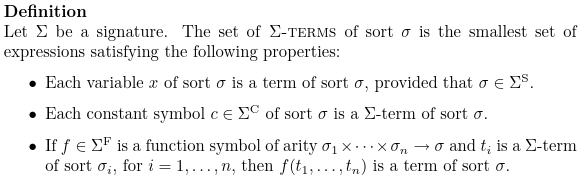
\includegraphics[width=\textwidth]{resources/zarba.png}
    \end{frame}

    \begin{frame}[fragile]{Klasická negace pro kódování robustnosti\\Symbol \texttt{on}}

\begin{lstlisting}[language=Prolog, numbers=none]
on(L, N) :-
    -B <= #sum{ W,M : on(L-1, M), weight(L, M, N, W) },
    bias(L, N, B).
\end{lstlisting}
        \hrule
\begin{lstlisting}[language=Prolog, numbers=none]
on(L, N) :-
    -B <= #sum{ W,M :  on(L-1, M), weight(L, M, N, W) },
    bias(L, N, B).
-on(L, N) :-
    -B <= #sum{ W,M :  on(L-1, M), weight(L, M, N, W) },
    bias(L, N, B).
\end{lstlisting}
    \end{frame}

\begin{frame}{Hammingova vzdálenost $r=0,1,2,3,4$}
\begin{figure}[p]%
    \begin{tikzpicture}[scale=1]
        \begin{loglogaxis}[
                legend entries={M1$\neg$, M1, M2$\neg$, M2, M3$\neg$, M3},
                legend pos=outer north east,
                cycle multi list={
                    color list\nextlist
                    mark=*
                },
                axis equal,
                xlabel={velikost oblasti vstupů},
                ylabel={čas [s]},
            ]
            \foreach \modelArch/\modelNum in \modelsSmall{
                \addplot+[
                    x filter/.expression={ln(hamming(100, x))},
                    y filter/.expression={\strequal{\thisrow{model}}{models/mnist_bnn_\modelArch/} ? ln(y) : nan}
                ] table [x=hamming-distance, y=Time, meta=color] {negation_hamming.csv};
                \addplot+[
                    x filter/.expression={ln(hamming(100, x))},
                    y filter/.expression={\strequal{\thisrow{model}}{models/mnist_bnn_\modelArch/} ? ln(y) : nan}
                ] table [x=hamming-distance, y=Time, meta=color] {hamming_big_add.csv};
            }
        \end{loglogaxis}
    \end{tikzpicture}
\end{figure}
\end{frame}
\end{document}
